\section{Monodisperse particle tracking}
\begin{frame}{Monodisperse particle tracking}
	\begin{columns}[T]
	\column{0.3\textwidth}
	Original image\\
	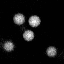
\includegraphics[width=\textwidth]{dillute_raw}
	
	\bigskip
	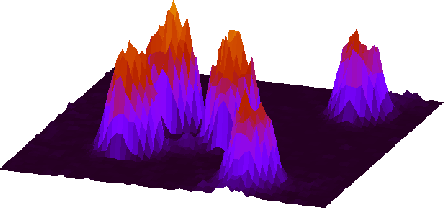
\includegraphics[width=\textwidth]{dillute_raw_gp_raster}
	\column{0.3\textwidth}
	Blurred\\
	
\includegraphics[width=\textwidth]{dillute_filtered}
	
	\bigskip
	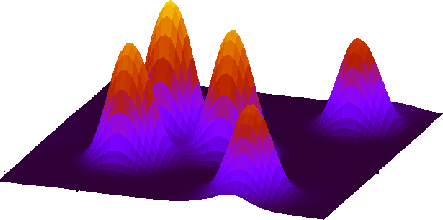
\includegraphics[width=\textwidth]{dillute_filtered_gp_raster}
	\column{0.3\textwidth}
	Local maxima\\
	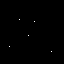
\includegraphics[width=\textwidth]{dillute_centers}
	
	\bigskip
	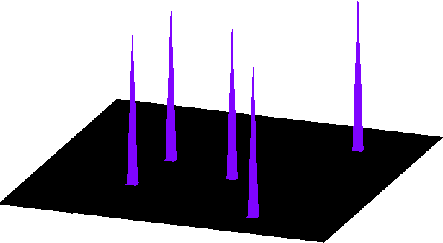
\includegraphics[width=\textwidth]{dillute_centers_gp_raster}
	\end{columns}
	
	
	Resolution up to $\SI{1/10}{px}$ via subpixel resolution methods.
	
	\bigskip
	
	\footnotesize{\citet{Crocker1996}}
\end{frame}

\begin{frame}{Monodisperse particle tracking}
	\begin{columns}[T]
	\column{0.3\textwidth}
	\centering
	Not enough blur\\
	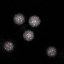
\includegraphics[width=\textwidth]{dillute_notblured}
	\column{0.3\textwidth}
	\centering
	Good blur\\
	\tikzsetnextfilename{not_blured_centers}
	\begin{tikzpicture}
		\node[inner sep=0, anchor=south west]{
\includegraphics[width=\textwidth]{dillute_filtered}};
		\fill[red!50!white] (9/64.0*\textwidth, 17/64.0*\textwidth) rectangle (10/64.0*\textwidth, 18/64.0*\textwidth);
		\fill[red!50!white] (19/64.0*\textwidth, 44/64.0*\textwidth) rectangle (20/64.0*\textwidth, 45/64.0*\textwidth);
		\fill[red!50!white] (28/64.0*\textwidth, 27/64.0*\textwidth) rectangle (29/64.0*\textwidth, 28/64.0*\textwidth);
		\fill[red!50!white] (34/64.0*\textwidth, 42/64.0*\textwidth) rectangle (35/64.0*\textwidth, 43/64.0*\textwidth);
		\fill[red!50!white] (51/64.0*\textwidth, 11/64.0*\textwidth) rectangle (52/64.0*\textwidth, 12/64.0*\textwidth);
	\end{tikzpicture}
	\column{0.3\textwidth}
	\centering
	Too much blur\\
	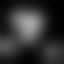
\includegraphics[width=\textwidth]{dillute_tooblured}
	\end{columns}
	\begin{itemize}
	\item We must choose \alert{the right} blurring radius.
	\item Ok for monodisperse particles
	\item Problematic for polydisperse
	\end{itemize}
\end{frame}

\begin{frame}{Same method with polydisperse particles}
	\begin{columns}[T]
	\column{0.3\textwidth}
	\centering
	{\strut{}Multiple centres}\\
	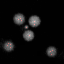
\includegraphics[width=\textwidth]{dillute_smaller_blur0_5}
	\column{0.3\textwidth}
	\centering
	{\strut{}Misplaced centres}\\
	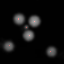
\includegraphics[width=\textwidth]{dillute_smaller_blur1}
	\column{0.3\textwidth}
	\centering
	{\strut{}Overlook small}\\
	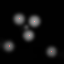
\includegraphics[width=\textwidth]{dillute_smaller_blur1_5}
	\end{columns}
	\begin{itemize}
	\item There is no \alert{right} blurring radius $\Rightarrow$ We always have errors.
	\item We cannot extract the sizes of the particles, important for the physics of the system.
	\begin{itemize}
		\item Volume fraction
		\item Neighbours
	\end{itemize}
	\end{itemize}
\end{frame}

\begin{frame}{Not better in 3D}
	\begin{center}
	\begin{tabular}{ccc}
	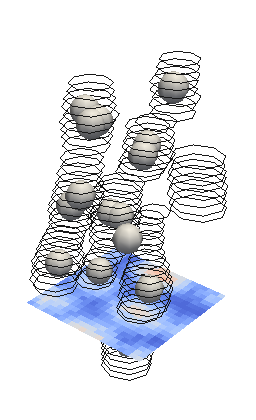
\includegraphics[width=0.18\textwidth]{comp3D_monoscale_r20_crop} & %
	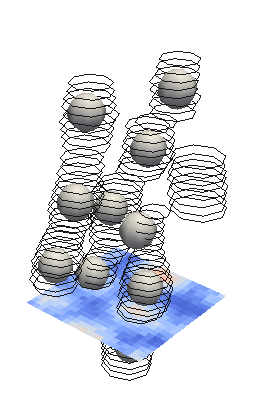
\includegraphics[width=0.18\textwidth]{comp3D_monoscale_r25_crop} & %
	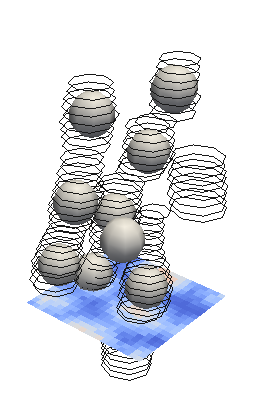
\includegraphics[width=0.18\textwidth]{comp3D_monoscale_r30_crop} \\ 
	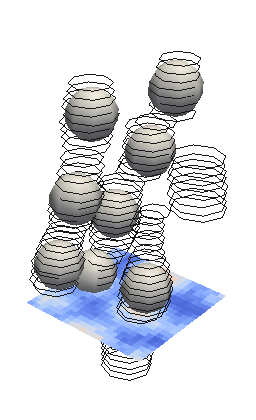
\includegraphics[width=0.18\textwidth]{comp3D_monoscale_r35_crop} & %
	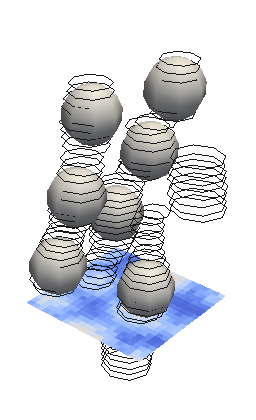
\includegraphics[width=0.18\textwidth]{comp3D_monoscale_r40_crop} & %
	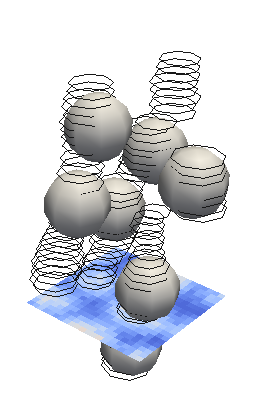
\includegraphics[width=0.18\textwidth]{comp3D_monoscale_r45_crop} \\ 
	\end{tabular} 
	\end{center}
\end{frame}

\section{Multiscale tracking}
\begin{frame}{Scale space}
	\footnotesize{Scale space,~\citet{Lindeberg1993}\\ Scale-invariant feature transform,~\citet{Lowe2004}}
	
	\tikzsetnextfilename{scale_space}%
	\begin{tikzpicture}[%
		minus/.style={
			shape=circle, draw, inner sep=0, %
			text height=1.5ex,text depth=.25ex,%
			node distance=0.5%
			},%
		]
		\begin{groupplot}[%
			group style={
				group size=2 by 1,%
				},%
			anchor=north,%
			width=0.5\textwidth,%
			xtick=\empty, ytick=\empty,%
			xlabel={position}, xlabel near ticks, ylabel near ticks, %
			no markers,
			title style={text height=1.5ex,text depth=.25ex, anchor=center},%
			]
			\nextgroupplot[%
				ylabel={intensity},%
				title={Increasing Gaussian blur},%
			]
				\addplot[black] table[x expr=\coordindex, y expr=\thisrowno{0}]{gaussians.txt};
				\addplot[blue] table[x expr=\coordindex, y expr=\thisrowno{1}-2]{gaussians.txt};
				\node at (current plot end) (g1) {};
				\addplot[blue!67!red] table[x expr=\coordindex, y expr=\thisrowno{2}-4]{gaussians.txt};
				\node at (current plot end) (g2) {};
				\addplot[blue!33!red] table[x expr=\coordindex, y expr=\thisrowno{3}-6]{gaussians.txt};
				\node at (current plot end) (g3) {};
				\addplot[red] table[x expr=\coordindex, y expr=\thisrowno{4}-8]{gaussians.txt};
				\node at (current plot end) (g4) {};
				
			\only<1>{
			\nextgroupplot[%
				title={Difference of Gaussians},%
				ymax=0.45,%
			]
				\addplot+[smooth, blue] table[x expr=\coordindex, y expr=\thisrowno{2}-\thisrowno{1}]{gaussians.txt};
				\node at (current plot begin) (DoG1) {};
				\addplot+[smooth, blue!67!red] table[x expr=\coordindex, y expr=\thisrowno{3}-\thisrowno{2}-0.2]{gaussians.txt};
				\node at (current plot begin) (DoG2) {};
				\addplot+[smooth, blue!33!red] table[x expr=\coordindex, y expr=\thisrowno{4}-\thisrowno{3}-0.4]{gaussians.txt};
				\node at (current plot begin) (DoG3) {};
			}
			\only<2>{
			\nextgroupplot[%
				title={Difference of Gaussians},%
			]
				\addplot+[smooth, blue] table[x expr=\coordindex, y expr=\thisrowno{2}-\thisrowno{1}]{gaussians.txt};
				\addplot+[smooth, blue!67!red] table[x expr=\coordindex, y expr=\thisrowno{3}-\thisrowno{2}]{gaussians.txt};
				\node at (current plot begin) (DoG2) {};
				\addplot+[smooth, blue!33!red] table[x expr=\coordindex, y expr=\thisrowno{4}-\thisrowno{3}]{gaussians.txt};
				\draw[->, thick] (rel axis cs:0.5,0.0015) -- (rel axis cs:0.5,0.075);
			}
				
		\end{groupplot}
		\only<1>{
		\node[minus, blue] (diff1) [left=of DoG1] {-};
		\draw [->, blue] (g1) -- (diff1);
		\draw [->, blue!67!red] (g2) -- (diff1);
		\draw [->, blue] (diff1) -- (DoG1);
		}
		\node[minus, blue!67!red] (diff2) [left=of DoG2] {-};
		\draw [->, blue!67!red] (g2) -- (diff2);
		\draw [->, blue!33!red] (g3) -- (diff2);
		\draw [->, blue!67!red] (diff2) -- (DoG2);
		\only<1>{
		\node[minus, blue!33!red] (diff3) [left=of DoG3] {-};
		\draw [->, blue!33!red] (g3) -- (diff3);
		\draw [->, red] (g4) -- (diff3);
		\draw [->, blue!33!red] (diff3) -- (DoG3);
		}
	\end{tikzpicture}
	
	\begin{itemize}
		\item The magnitude of the DoG should be maximized at the center of the blob.
		\item<2> The optimal scale, which depends on the size of the blob, should be detected.
	\end{itemize}
\end{frame}

\begin{frame}{Locating particles in both scale and space}
	\begin{columns}[T]
	\column{0.7\textwidth}
	\def\svgwidth{\columnwidth}
	\input{sift_octave1.pdf_tex}
	\def\svgwidth{\columnwidth}
	\input{sift_octave0.pdf_tex}
	\column{0.3\textwidth}
	\def\svgwidth{\columnwidth}
	\input{sift_localmin.pdf_tex}
	Minima of the DoG images are detected by neighbourhood search.
	\end{columns}
	
	\footnotesize{\citet{Lindeberg1993, Lowe2004}}
\end{frame}



\begin{frame}{Optimal scale}
	For a binary disk of radius $R$, the DoG response is minimum for a scale $\sigma^{*} \propto R$. The proportionality constant is known analytically.
	
	\begin{columns}[T]
	\column{0.3\textwidth}
	\tikzsetnextfilename{binary_sphere}%
	\begin{tikzpicture}
		\usebeamercolor{palette primary}
		\fill[black] (-0.5\columnwidth,-0.5\columnwidth) rectangle (0.5\columnwidth, 0.5\columnwidth);
		\fill[white] (0,0) circle (0.25\columnwidth);
		\draw[->, fg, thick] (0,0) -- (0.25\columnwidth, 0);
		\node[below, fg] at (0.125\columnwidth, 0) {$R$};
	\end{tikzpicture}
	\column{0.7\textwidth}
	\tikzsetnextfilename{scale2radius}%
	\begin{tikzpicture}
		\begin{axis}[
			width=0.8\columnwidth,%
			xmin=0, ymax=0, xmax=5, %
			xlabel=$R/\sigma^*$, ytick={0},%
			ylabel={DoG response}, ylabel near ticks, %
			no marks,%
			]
			\addplot+[smooth] {exp(-x^2/2) - exp(-x^2/2/2^(2/3))};
		\end{axis}
	\end{tikzpicture}
	\end{columns}
\end{frame}

\begin{frame}{Isolated sphere}
	\tikzsetnextfilename{isolated_sphere}%
	\begin{tikzpicture}
	\pgfplotsset{cycle list name=black white, clip marker paths=true,}
	\begin{axis}[%
		name=size,
		width=0.5\columnwidth,%
		height=0.5\columnwidth,%
		xlabel={Input radius}, ylabel={Output radius},%
		extra x ticks={3.47}, extra x tick labels={}, extra tick style={grid=major},%
		ytick={2,4,...,14},
		axis background/.style={fill=white},%
		]
		\addplot+[only marks, mark size=0.5, mark=o] table [x index=0, y expr ={\thisrowno{1}}] {multiscale_relative_sizes.out};
		\addplot+[no marks, domain=1.5:14] {x};
	\end{axis}
	\begin{axis}[%
		name=errorsize,
		at={(0.5\columnwidth,0)},%
		width=0.5\columnwidth,%
		height=0.5\columnwidth,%
		xlabel={Input radius (px)}, ylabel={$R$ relative error (\%)},%
		extra x ticks={3.47}, extra x tick labels={}, extra tick style={grid=major},%
		extra y ticks={0}, extra y tick labels={},%
		ylabel near ticks,
		]
		\addplot table [x index=0, y expr ={100*(\thisrowno{1}/\thisrowno{0}-1)}] {multiscale_relative_sizes.out};
	\end{axis}
	\end{tikzpicture}
\end{frame}

\begin{frame}{Two spheres}
	%\tikzset{external/force remake=false}
	\begin{columns}[c]
	\column{0.55\textwidth}
	\tikzsetnextfilename{two_spheres}%
	\begin{tikzpicture}
	\begin{groupplot}[%
		group style={
				group size=1 by 2,%
				},%
		height=0.5\textheight,%
		width=\columnwidth,%
		xlabel={$r_{ij}$ (px)}, 
		xmin=8, xmax=18, xtick={8,...,17},%
		extra tick style={grid=major},%
		]
		\nextgroupplot[%
			ylabel={$r_{ij}$ error (\SI{0.01}{px})},%
			extra y ticks={0}, extra y tick labels={},%
			]
		\addplot table [x index=0, y expr ={(\thisrowno{2}-\thisrowno{1}-\thisrowno{0})*100}] {close_neighbours3D.out};
		\draw (axis cs:12,-6) circle[radius=0.05\textwidth] (axis cs:16,-6) circle[radius=0.05\textwidth];
		\draw[dashed] (axis cs:12,-6) -- (axis cs:12,-9) (axis cs:16,-9) -- (axis cs:16,-6);
		\draw[<->] (axis cs:12,-9) -- (axis cs:16,-9) node[midway, above] {$r_{ij}$};
		\draw[->] (axis cs:11.05,-6) -- +(0,0.05\textwidth,0) node[midway, left] {\SI{4}{px}};
		\draw[->, very thick] (axis cs:16,-6) -- (axis cs:14,-6);
	
	\nextgroupplot[
		ylabel={$R$ (px)},%
		extra y ticks={4}, extra y tick labels={},%
		legend style={legend pos=south east}
		]
		\addplot table [x index=0, y index=4] {close_neighbours3D.out};
		\addplot+[mark=square] table [x index=0,y index=6] {close_neighbours3D.out};
		\legend{No correction, One iteration};
	\end{groupplot}
	\end{tikzpicture}
	\column{0.45\textwidth}
	Error at contact $\approx \SI{0.1}{px}$, like monodisperse tracking.
	
	\bigskip
	
	The DoG response at the center of particle $i$ is a superposition of the contribution of each (neighbouring) particle.
	\[
	%\forall i,\quad 
	DoG_i = \sum_j DoG(r_{ij}, R_j)
	\label{eq:superpos}
	\]
	\end{columns}
\end{frame}

\begin{frame}{Many particles}
	%\tikzset{external/force remake=false}
	Monodisperse simulation data from John Russo written as a 3D image with black margins.
	\tikzsetnextfilename{many_particles}
	\begin{tikzpicture}
	\pgfplotsset{cycle list name=black white, clip marker paths=true,}
	\begin{axis}[%
		name=finite,
		at={(0,-1.35\columnwidth)},%
		height=0.5\columnwidth,%
		width=\columnwidth,%
		area legend,
		const plot, no marks,%
		xlabel={$R$ (px)}, ylabel={Size distribution},%
		%xmin=8, xmax=18,%
		extra tick style={grid=major},%
		extra x ticks={5.298}, extra x tick labels={},%
		ymin=0,%		
		legend style={legend pos=north west, cells={anchor=west}}
		]
		\addplot+[pattern=north west lines] file {john_exact_mono_large_init.hist} \closedcycle;
		\addplot+[gray, fill=gray, semitransparent] file {john_exact_mono_large_cor1.hist} \closedcycle;
		\addplot+[pattern=dots] file {john_exact_mono_large_cor2.hist};
		\legend{No correction, One iteration, Two iterations};
		\draw[decorate,decoration=brace] (axis cs:4.75, 200) -- (axis cs:5.05, 200) node[midway, above] {edges};
	\end{axis}
	\end{tikzpicture}
\end{frame}


%\tikzset{external/force remake=true}
\begin{frame}{Deconvolution}
	\begin{columns}[c]
	\column{0.66\textwidth}
	$y = x \star h + \epsilon$ with $h$ the point spread function.
	\tikzsetnextfilename{deconvolution}%
	\begin{tikzpicture}
		\begin{groupplot}[%
		group style={
				group name=pics,
				group size=3 by 1,%
				horizontal sep=0.0075\textwidth,
				vertical sep=0.0075\textwidth,
				},%
		width=0.3\textwidth,%
		height=0.33\textwidth,%
		xmin=0,xmax=50,ymin=0,ymax=55,%
		axis lines=none,%
		scale only axis=true,%
		point meta=explicit symbolic,%
		scatter/@pre marker code/.code={%
        	\pgfmathparse{10*\pgfplotspointmetatransformed*\pgfplotsunitxlength}%
        	%\pgfplotstransformcoordinatex{\pgfplotspointmetatransformed}
            \def\markopts{mark=o,black,mark size=\pgfmathresult}%
            \expandafter\scope\expandafter[\markopts]
            },%
        scatter/@post marker code/.code={\endscope} 
		]
		\nextgroupplot[title={Original}]
			\addplot graphics [xmin=0,xmax=50,ymin=0,ymax=55]{Zelong_original};
		\nextgroupplot[title={Blurred}]
			\addplot graphics [xmin=0,xmax=50,ymin=0,ymax=55]{Zelong_blurred};
			\addplot+[only marks, scatter] table [x index=1, y expr={55-\thisrowno{2}}, meta index=3] {Z_elong.xyz};
		\nextgroupplot[title={Deconvolved}]
			\addplot graphics [xmin=0,xmax=50,ymin=0,ymax=55]{Zelong_deconvolved};
			\addplot+[only marks, scatter] table [x index=1, y expr={55-\thisrowno{2}}, meta index=3] {Z_elong_deconv.xyz};
		\end{groupplot}
	\end{tikzpicture}
	\begin{itemize}
	\item If the system is isotropic, the spectrum along $z$ must be the same as the spectrum along $x$ ou $y$.\\ $\Rightarrow$ Possible to measure the \textsc{psf}.
	\item No need to deconvolve the noisy original image, we can use the first Gaussian blurred version.
	\end{itemize}
	
	
	\column{0.33\textwidth}
	\tikzsetnextfilename{rdf_deconv}%
	\begin{tikzpicture}
		\begin{axis}[%
			anchor=outer south west,
			width=\columnwidth,%
			height=0.9\textheight,%
			xlabel = {$r$ [\si{\micro\metre}]}, ylabel={$g(r)$},%
			xlabel near ticks, ylabel near ticks,
			xmin=0,xmax=4,ymin=0,%
			no marks,%
			]
			\addplot file {cp0.34.rdf};
			\addplot file {cp0.34_deconv.rdf};
		\end{axis}
	\end{tikzpicture}
	\end{columns}
\end{frame}
